% !TEX root = main.tex

\section{空间域图像增强}
图像增强目的是提高图像在特定应用领域的视觉质量,包括光滑、锐化、提取边缘、反转、去噪以及各种滤波等。

空间域图像增强的是直接对图像的像素进行操作,基本关系式可表示如下:
\[g(x,y)=T(f(x,y))\]

\subsection{基本灰度变换}
\begin{itemize}
\item 基本灰度函数:线形、对数、幂次
\begin{figure}[H]
\centering
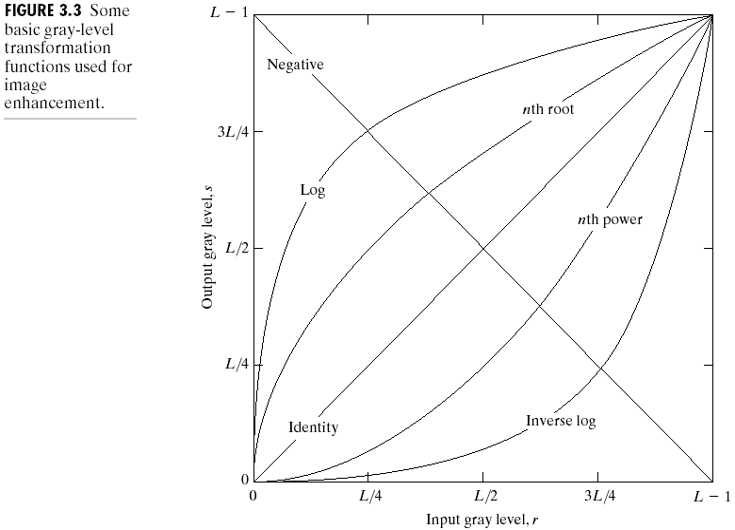
\includegraphics[width=0.6\linewidth]{fig/enhancement.png}
\end{figure}
\item 图像反转变换:$s=L-1-r$,人眼的一个特点就是在背景相对光亮时对灰度层次有较好的分辨能力。
\begin{figure}[H]
\centering
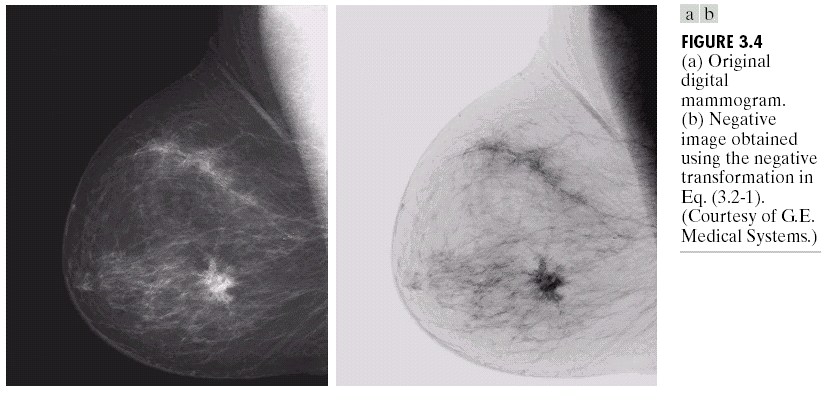
\includegraphics[width=0.6\linewidth]{fig/trans-inverse.png}
\end{figure}
\item 对数变换:$s=c\log(1+r)$,$c$是常数,$r\geq 0$,适合大范围的数据压缩。
任何具有对数函数曲线形状的变换都可以完成灰度的压缩和扩展功能。 
\begin{figure}[H]
\centering
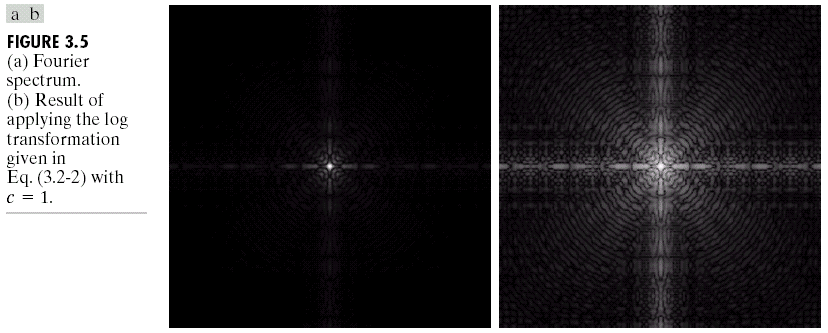
\includegraphics[width=0.6\linewidth]{fig/trans-log.png}
\end{figure}
\item 幂次变换:$s=cr^\gamma$,$c$和$\gamma$都为正常数
\begin{figure}[H]
\centering
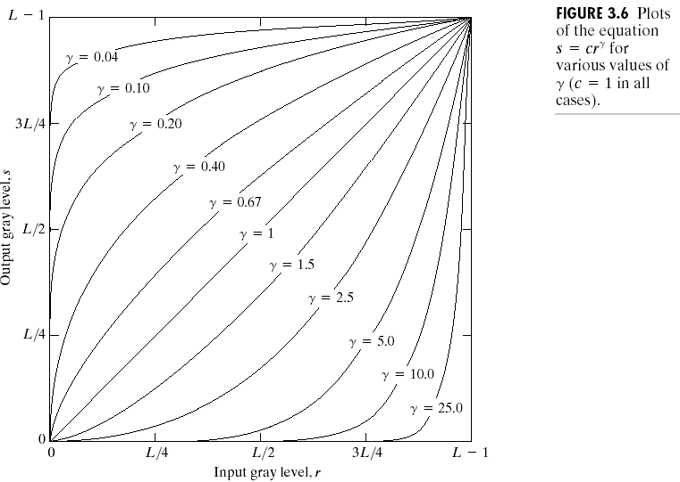
\includegraphics[width=0.6\linewidth]{fig/trans-power.png}
\end{figure}
伽马校正:大量的图像设备如捕捉卡、打印机、数码相机以及显示装置的响应(输出)就对应一个幂函数,通常称这个幂函数的指数为gamma。纠正这个幂次响应的处理称为伽玛校正(gamma correction)。
\begin{figure}[H]
\centering
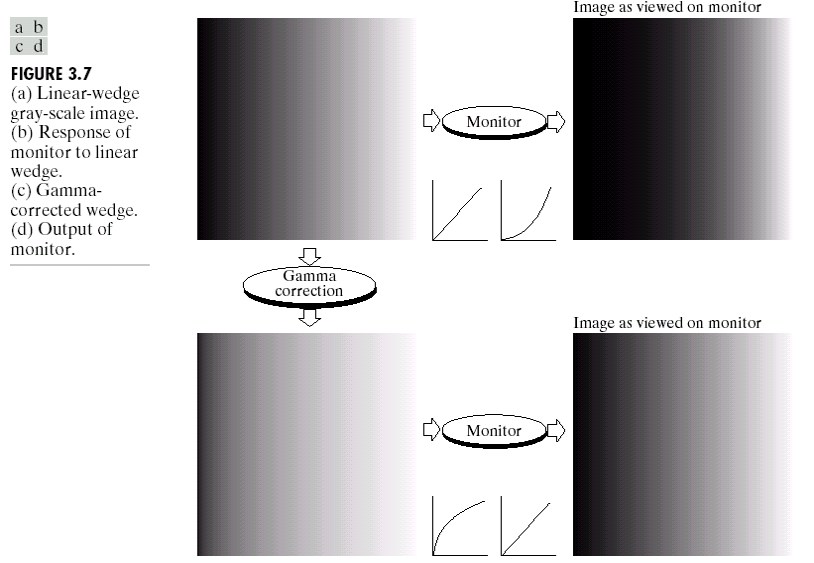
\includegraphics[width=0.6\linewidth]{fig/trans-gamma.png}
\end{figure}
在一般的图像处理软件中,几乎都有伽玛校正的功能。这个功能可用于调整图像的对比度。如果图像偏暗,有些低灰度值的细节被掩盖时,可考虑用指数$\gamma<1$的伽玛校正;反之,$\gamma>1$的校正对那些被“漂白”的细节会起作用。
\item 分段线性变换
\begin{figure}[H]
\centering
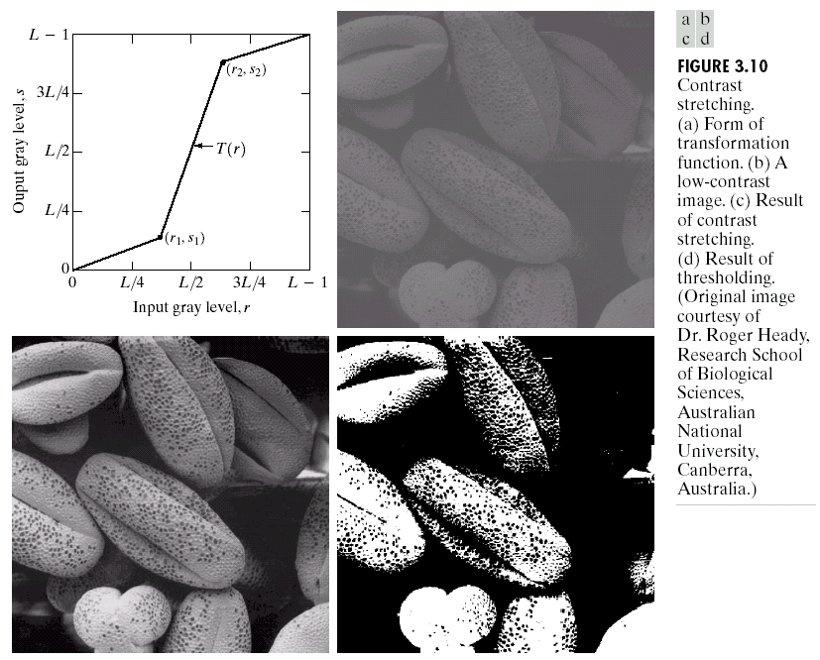
\includegraphics[width=0.6\linewidth]{fig/trans-by-cases.png}
\end{figure}
\item 灰度切割:在图像中提高特定灰度的亮度
\begin{figure}[H]
\centering
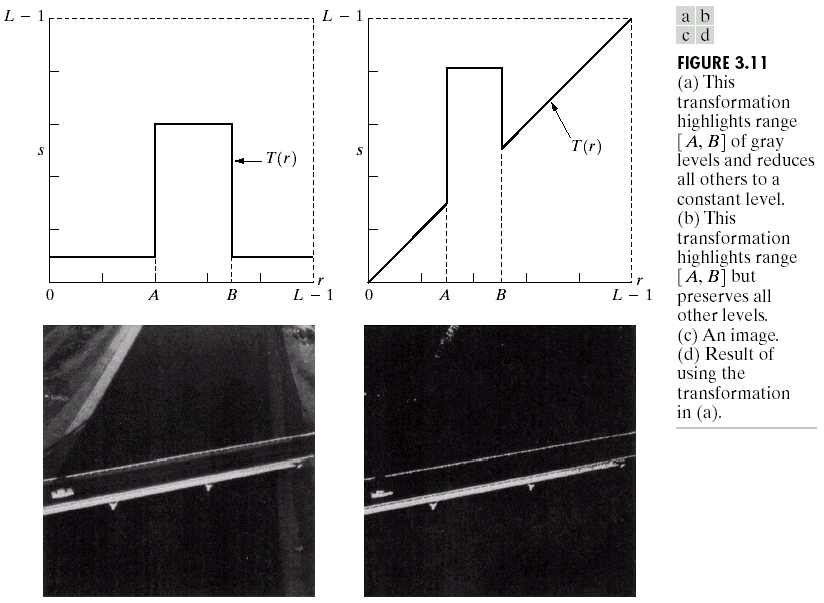
\includegraphics[width=0.6\linewidth]{fig/trans-cut.png}
\end{figure}
\end{itemize}

位图切割:8位灰度图象可以分割成8个位面,每个是一个二值图像。
\textbf{高位}表示了\textbf{重要的信息},\textbf{低位}给出了\textbf{不同程度的细节}。
\begin{figure}[H]
\centering
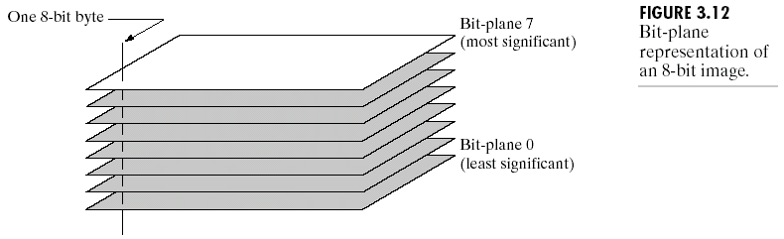
\includegraphics[width=0.6\linewidth]{fig/bitmap.png}
\end{figure}

位图的作用
\begin{itemize}
	\item 信息隐藏:藏在中间位,低位会被丢弃,高位太清楚
	\item 视频传输:先传高位,再传低位,逐渐清晰
\end{itemize}

\subsection{直方图}
\begin{definition}[直方图]
灰度级别为$[0,L-1]$(直方图一定从0开始!)。数字图像直方图是离散函数$h(r_k)=n_k$,其中$r_k$是第$k$级灰度,$n_k$是图像中灰度级为$r_k$的像素个数(频数)。
除以总数$n$就得到归一化的直方图。
\end{definition}

\subsubsection{直方图均衡化}
有亮度差才能看到细节,均衡分布
\begin{figure}[H]
\centering
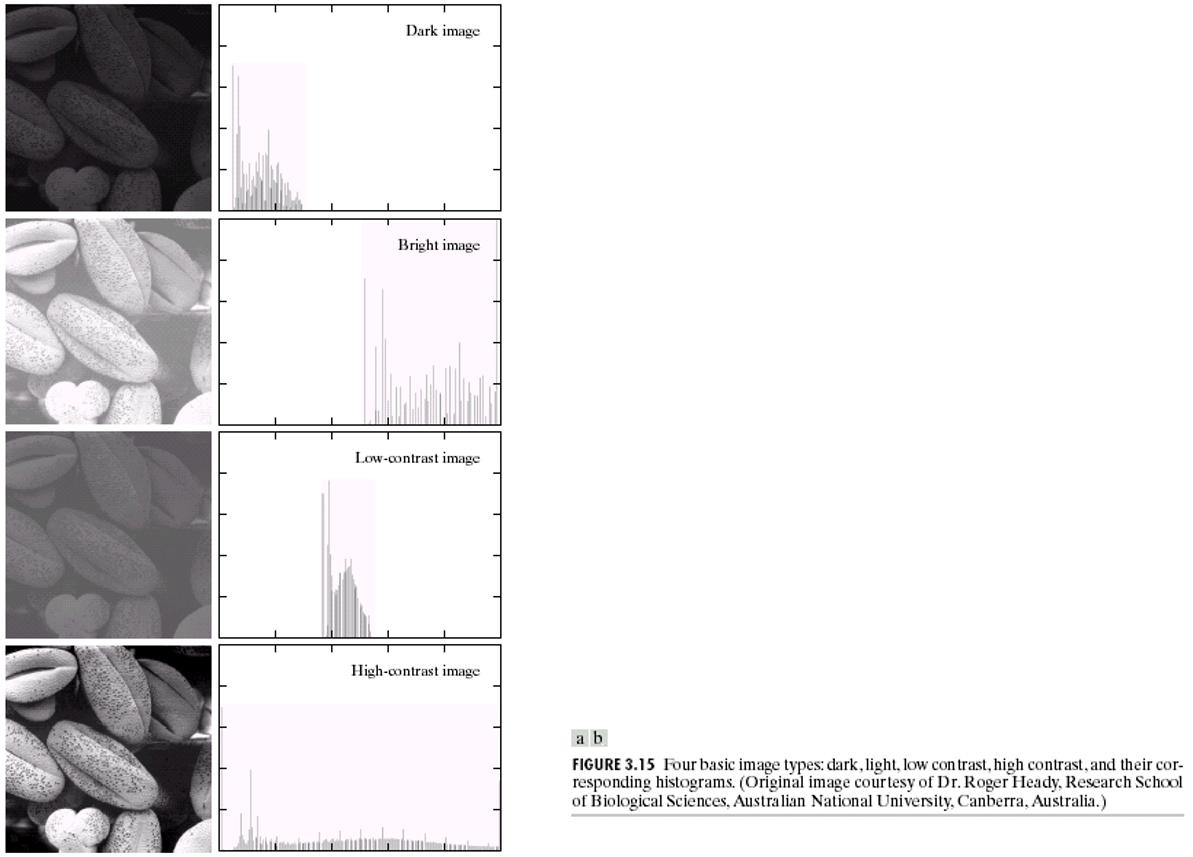
\includegraphics[width=0.6\linewidth]{fig/histogram-quality.png}
\end{figure}

直方图均衡化/线性化则是寻求一种变换使得变换后的图像具有尽可能均匀分布的直方图,用于图像增强最大的特点是自动化,有强大的适应性强的功能。
步骤如下:
\begin{itemize}
	\item 概率$p_r(r_k)=n_k/n,k=0,1,2,\ldots,L-1$
	\item 累计分布函数(PDF)
	\[P(r_k)=\sum_{j=0}^k p_r(r_j)=\sum_{j=0}^k\frac{n_j}{n},k=0,1,2,\ldots,L-1\]
	\item 变换函数
	\[s_k=T(r_k)=(L-1)\cdot\sum_{j=0}^k\frac{n_j}{n},k=0,1,2,\ldots,L-1\]
	\item 将$s_k$四舍五入转换为标准灰度级别,如有相同$\lceil s_k\rceil$则合并
\end{itemize}
\begin{figure}[H]
\centering
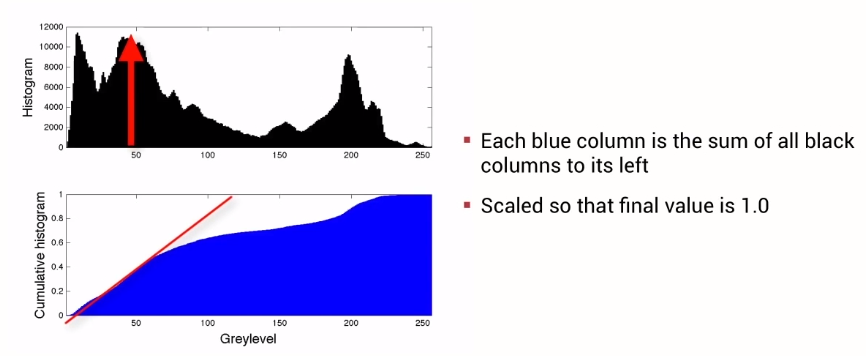
\includegraphics[width=0.8\linewidth]{fig/histogram-normalization.png}
\end{figure}
\begin{analysis}
若$r$为离散型随机变量,$T(r)$为单调递增函数($T^{-1}$存在且单调),且$s=T(r)$,则由概率论有
\[p_s(s)=p_r(r)\pd{r}{s}\Big|_{r=T^{-1}(s)}=p_s(T^{-1}(s))|T^{-1}(s)|\]
考虑变换函数为$r$的累积分布函数(CDF)
\[s=T(r)=\intabu{0}{r}{p_r(\omega)}{\omega}\]
对$s$求导并代入上面的式子可得$p_s(s)=1$,故实现均衡。
算法实际上就是求累积分布函数,使得原本亮度小的像素能够映射到亮度大的空间。
\end{analysis}

% Project1
% 黑白图像
% 1. 获取直方图 并均衡
% 2. gamma校正 亮->暗 暗->亮

\subsubsection{直方图匹配}
当两幅图像比对时,通常要使其直方图形式一致(如不同光照条件下的同一场景)。

做法是使两幅图像均衡化后的结果相同,即
\[\begin{aligned}
s&=T(r)=\intabu{0}{r}{p_r(w)}{w}\\
s&=G(z)=\intabu{0}{z}{p_z(t)}{t}
\implies z&=G^{-1}(s)=G^{-1}(T(r))
\end{aligned}\]

\begin{definition}[$n$阶矩]
设$p_r(r_k)=n_k/n$,则$r$的第$n$阶中心矩为
\[\mu_r(r_k)=\sum_{i=0}^{L-1}(r_i-m)^np(r_k)\]
其中$m=\sum_{i=1}^{L-1}r_ip(r_i)$为$r$的平均值。
特别地,当$n=2$时为方差。
\end{definition}


\subsection{空间滤波基础}
滤波的概念来自信号处理中的傅里叶变换,空间滤波指的是直接对图像像素进行处理的操作。
滤波器(filter)有时也叫掩模(mask)、核(kernel)、模板(template)或窗口(window)。

\subsubsection{线性滤波}
空间域线性滤波基本公式:
\[g(x,y)=\sum_{s=-a}^a\sum_{t=-b}^b w(s,t)f(x+s,y+t)\]

一个$M\times N$的滤波器$w(x,y)$与图像$f(x,y)$的相关操作定义为
\[w(x,y)\circ f(x,y)=\sum_{s=-a}^a\sum_{t=-b}^b w(s,t)f(x+s,y+t)\]
一个$M\times N$的滤波器$w(x,y)$与图像$f(x,y)$的卷积定义为
\[w(x,y)*f(x,y)=\sum_{s=-a}^a\sum_{t=-b}^b w(s,t)f(x+s,y+t)\]

空间滤波对边界的处理方法
\begin{itemize}
	\item 重复边缘值
	\item 卷绕输入图像
	\item 补零
	\item 勿略
\end{itemize}

常用的光滑滤波器(左侧是均值滤波)
\begin{center}
\begin{tabular}{|c|c|c||c|c|c|}\hline
1/9 & 1/9 & 1/9 & 1/16 & 1/8 & 1/16\\\hline
1/9 & 1/9 & 1/9 & 1/8 & 1/4 & 1/8 \\\hline
1/9 & 1/9 & 1/9 & 1/16 & 1/8 & 1/16\\\hline
\end{tabular}
\end{center}

一般公式
\[g(x,y)=\frac{\sum_{s=-a}^a\sum_{t=-b}^b w(s,t)f(x+s,y+t}{\sum_{s=-a}^a\sum_{t=-b}^b w(s,t)}\]

\subsubsection{非线性滤波}
排序统计滤波器是一种非线性的、 非卷积滤波器。
排序统计滤波器在滤波器包围的像素范围内排序,然后由统计排序结果决定的值代替中心像素的值。
按排序输出的位置分,可分为:中值滤波、最大值滤波、最小值滤波。